\documentclass[times, 10pt, twocolumn]{article}
\usepackage{latex8}
\usepackage[dvips]{graphicx}
\usepackage[fleqn]{amsmath}
\usepackage{amsthm}
\usepackage{txfonts}
\usepackage{courier}
\usepackage{subfigure}
\usepackage{comment}
\usepackage{url}
\usepackage[square,numbers]{natbib}

\newcommand{\hd}{\emph{H+D}}
\newcommand{\hp}{\emph{Hpin}}
\newcommand{\dm}{\emph{Dmap}}

%-----------------------------------------
% need for camera-ready
%\pagestyle{empty}

%----------------------------------------


\title{Accelerating Traffic Simulation and Its Real-Time Challenges}

\author {
Manato Hirabayashi, Shinpei Kato, Masato Edahiro\\
\textit{Department of Information Engineering}\\
\textit{Nagoya University}\\
\and
Yuki Sugiyama\\
\textit{Department of Physics}\\
\textit{Nagoya University}\\
}

\begin{document}

\maketitle

%-----------------------------------------
% need for camera-ready
%\thispagestyle{empty}

\begin{abstract}
\end{abstract}

\section{Introduction}

Transportation systems underlie our industry and life as part of
societal infrastructure.
Economy depends highly on traffic flow.
Once a traffic jam occurs, for example, it could cause significant
economic damage through degradation of transport efficiency, energy
consumption, and environmental poisoning.
According to the Japanese government report a few years ago, economic
losses due to traffic congestion reach one hundred billion dollars per
year in Japan.
Albeit a major issue of transportation systems, the mechanism of traffic
jam is not well-explained in the literature.
What is particularly important is ``phantom jam'', which often happens
on freeways without any accident.
This phantom jam should be avoided by science, given that it is
a physical phenomenon but not one caused by human errors.
However, we are not aware of scientific and engineering solutions to
such real-world problems.

In physics, traffic flow is described by mathematical
models~\cite{Bando1995, Kerner1993, Nagel1992}.
While their mathematical expressions are not identical, they are all
compute-intensive procedures.
For example, traffic simulation based on the Optimal Velocity (OV)
model~\cite{Bando1995} computes locations and velocities of agents every
sampling period, solving OV equations. 
Specifically, the location $x_n$ of the $n$th agent is described by the
following equation, where $\Delta x_n = x_{n+1} - x_n$ is a distance to
a preceding agent, $a$ is a sensitivity, and $V()$ is an optimal
velocity function:
\begin{eqnarray}
 \label{eqn:ov}
 \frac{d^2 x_n}{d t^2} = a \left\{V(\Delta x_n) - \frac{d x_n}{d t}\right\}.
\end{eqnarray}

Applying a large number of agents to simulation using the above formula,
it is apparent that computational workload increases exponentially.
In fact, the above formula considers only one dimension, which restricts
applications of simulation to freeway traffic flows, powder flows,
molecular motors, and so on.
Making it multi-dimensional further increases computational workload,
while allowing more complicated simulations, such as traffic networks,
internet packet flows, evacuation routes, and herd formations of
animals, to use similar optimal velocity models.
Given a scale of million agents in the real world, traffic
simulation should be supported by powerful computer systems.

Deployment of traffic simulation may require real-time feedback from the
real world.
This turns out to be a cyber-physical systems (CPS) problem.
Real-time traffic simulation is another challenging issue, where
the rate and the preciseness of simulation must be traded to meet the
requirement of a given scenario.
For instance, evacuation may want very high rate simulation, sacrificing
the preciseness of simulation to some extent.
Unfortunately, none of those challenges has been explored yet, largely
due to a lack of multidisplinary research collaborations between physics
and computer science.

This paper explores how to accelerate traffic simulation using the
state-of-the-art parallel computing technology.
In particular, we use the graphics processing unit (GPU), which
integrates hundreds of cores on a chip.
Recent GPUs are becoming more and more suitable for general-purpose
data-parallel applications.
The traffic simulation program used in this paper applies
Equation~\eqref{eqn:ov} to a large number of agents.
The resulting workload is highly data-parallel and compute-intensive,
which can be nicely offloaded on to the GPU.
We also identify the bottleneck in accelerating our traffic simulation
program using the GPU, and provide some insight into its solution.

\section{Assumption}
\label{sec:assumption}

\begin{enumerate}
 \item Initalize the time $t$, and set the initial values of $x_n(t)$
       (also $y_n(t)$ and $z_n(t)$, if necessary for multidimensional
       versions).
 \item Increase the time $t$ by the sampling period $\Delta t$.
 \item Compute the location $x_n(t)$ (also $y_n(t)$ and $z_n(t)$, if
       necessary for multidimensional versions), and the velocity
       $v_x(t)$ at time $t$ for each agent $A_n$, using the OV model.
 \item Go back to Step 2, if the simulation time is expired.
 \item Exit the program.
\end{enumerate}

Note that Step 3 explots a lot of loop procedures to derive the
locations and velocities of agents.
This part can be accelerated by the GPU.

\section{GPU Implementation}
\label{sec:gpu_implementations}

GPU performance is dominated by the program design.
GPU-accelerated programs are typically divided into two pieces of code.
The CPU code plays a role of a master thread that controls the program
flow.
The GPU code, on the other hand, spawns a bunch of worker threads to
execute compute-intensive parts of the program in parallel, thus
accelerating the overall program.
What is often argued to optimize performance is how to parallelize the
program into threads.

In order to optimize GPU performance, however, we need to make a
difficult decision about when to offload on to the GPU.

\begin{figure}[t]
\centering
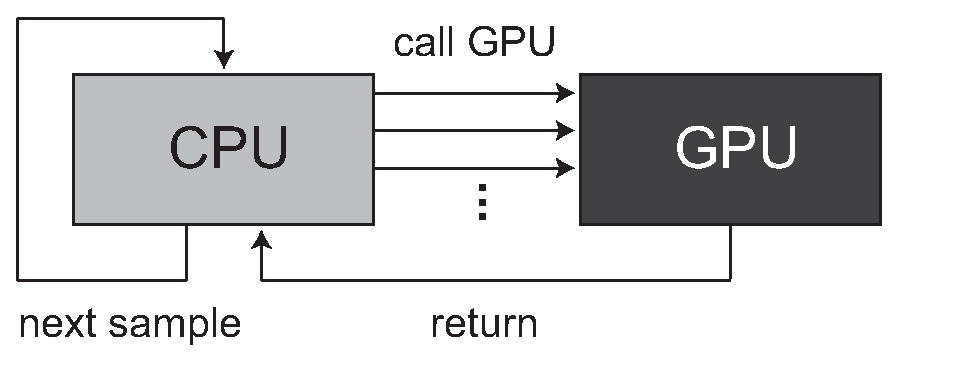
\includegraphics[width=0.4\textwidth]{eps/sample-in-cpu.eps}
\caption{Sampling by the CPU.}
\label{fig:sample-in-cpu}
\end{figure}

\begin{figure}[t]
\centering
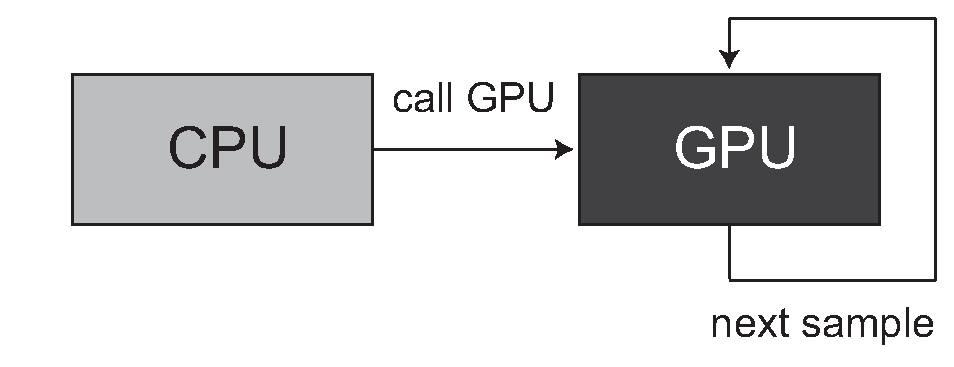
\includegraphics[width=0.4\textwidth]{eps/sample-in-gpu.eps}
\caption{Sampling by the GPU.}
\label{fig:sample-in-cpu}
\end{figure}


\section{Evaluation}
\label{sec:evaluation}

\begin{figure}[t]
\centering
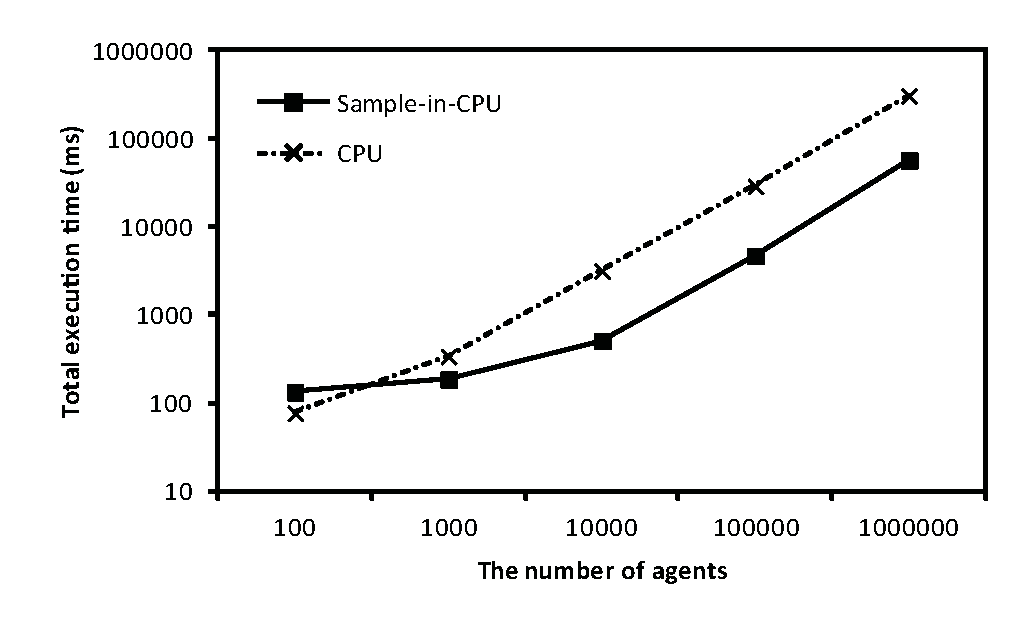
\includegraphics[width=0.5\textwidth]{eps/eval_accel.eps}
\caption{Acceleration of traffic simulation.}
\label{fig:eval_accel}
\end{figure}

\begin{figure}[t]
\centering
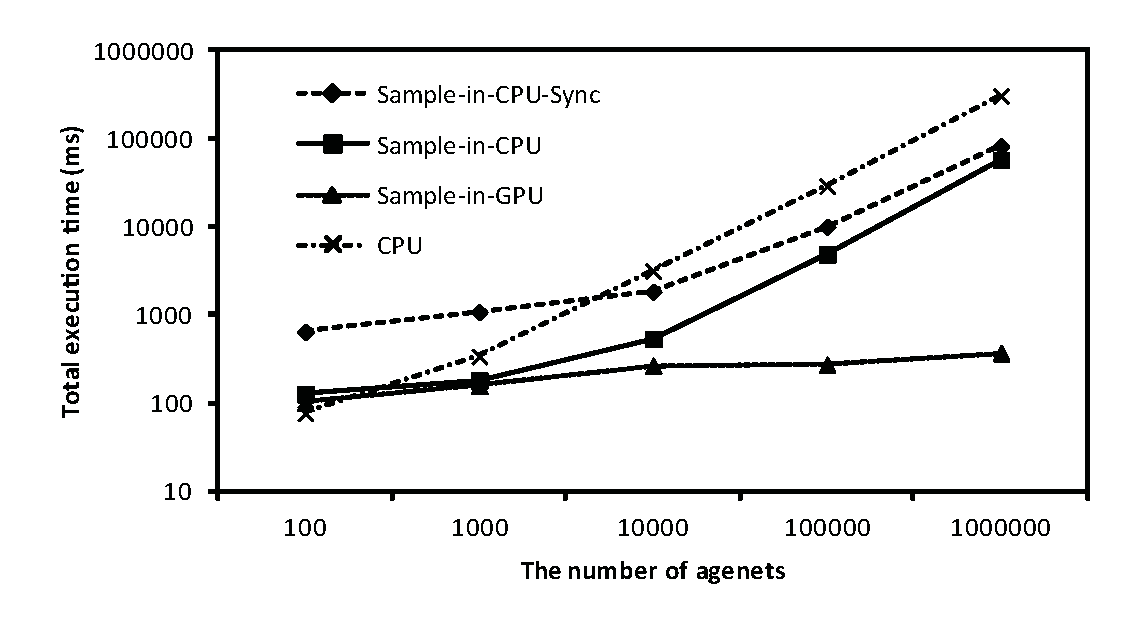
\includegraphics[width=0.5\textwidth]{eps/eval_nosync.eps}
\caption{Impact of synchronization.}
\label{fig:eval_nosync}
\end{figure}

\begin{figure}[t]
\centering
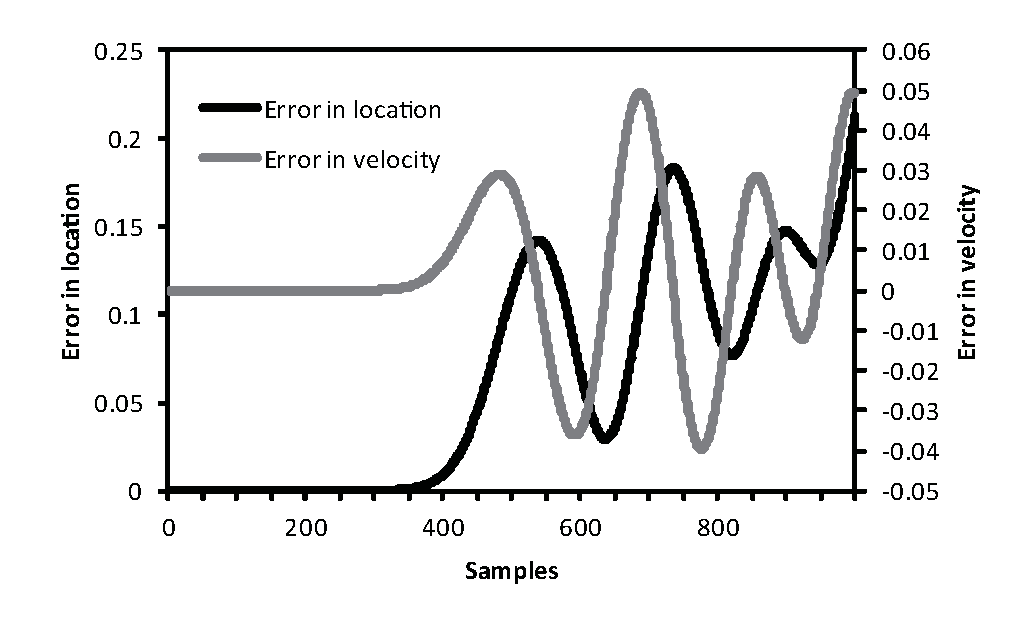
\includegraphics[width=0.5\textwidth]{eps/eval_error.eps}
\caption{Error in location and velocity due to imprecise synchronization.}
\label{fig:eval_error}
\end{figure}

\section{Conclusion}
\label{sec:conclusion}

Gdev~\cite{Kato2012}.

\bibliographystyle{plain}
{\footnotesize
\bibliography{references}
}

\end{document}
